\documentclass[a4paper, 12pt]{article}
\usepackage[utf8]{inputenc}
\usepackage{myshortcuts}
\usepackage{a4wide}
\usepackage{mhchem}
\usepackage{siunitx}
\usepackage{csquotes}
\usepackage{enumitem}
\usepackage{etoolbox}
\usepackage[british]{babel}
\usepackage[labelfont=bf]{caption}
\usepackage[style=numeric,backend=biber]{biblatex}

\DeclareSIUnit{\molar}{M}

\addbibresource{mysources.bib}

\title{
\textbf{Chemistry Internal Assessment}\\
\bigskip
What effect does varying the concentration have on the rate of decomposition of \ce{H2O2} in presence of \ce{Fe^3+} ions?
}
\author{Jingjie YANG}
\date{}

\begin{document}
\maketitle

\section{Background Information}
$$\ce{H2O2(aq) ->[Fe^3+] 2H2O(l) + O2(g)}$$

\section{Research Question}
\paragraph{Hypothesis}

\section{Variables}
\paragraph{Independent variable:}
concentration of \ce{H2O2}

\paragraph{Dependent variable:}
initial rate of change in gas pressure

\paragraph{Controlled variables:}
\begin{itemize}
    \item volume of reaction mixture
    \item concentration of \ce{FeCl3} catalyst
    % TODO check if these should be included if to be talked in evaluation
    \item temperature of reaction mixture
    \item volume of test tube
\end{itemize}

\section{Materials}
\subsection{Apparatus}
\begin{itemize}
    \item \SI{1}{\L} beaker
    \item \SI{18x150}{\mm} glass test tubes
    \item one-hole rubber stopper
    \item tubing with two Luer-lock connectors
    \item LabQuest
    \item Vernier temperature probe (range: \num{-40} to \SI{135}{\celsius}; accuracy: \SI{+-0.2}{\celsius} \autocite{vernier_temperature})
    \item Vernier gas pressure sensor (range: \num{0} to \SI{210}{\kPa}; accuracy: \SI{+-4}{\kPa} \autocite{vernier_gas_pressure})
    \item three \SI{5.00}{\mL} graduated pipettes (precision: \SI{+-0.05}{\mL}) with bulbs
\end{itemize}

\subsection{Chemicals}
\begin{itemize}
    % TODO calculate molar concentration
    \item \SI{80}{\mL} of \SI{3}{\percent} \ce{H2O2}
    \item \SI{30}{\mL} of \SI{0.1}{\molar} \ce{FeCl3}
    \item \SI{80}{\mL} of distilled water
\end{itemize}
\paragraph{Safety} 
% TODO add safety information
Although \SI{3}{\percent} \ce{H2O2} is classified as non-hazardous \autocite{safety_h2o2}, \SI{0.1}{\molar} \ce{FeCl3} is identified to be irritant and corrosive upon immediate skin or eye contact \autocite{safety_fecl3}. Goggles, gloves, and a lab coat must be worn.

\section{Method}
\begin{enumerate}
    \item Set up a water bath with a \SI{1}{\L} beaker to immerse a test tube with room-temperature water --- see \cref{fig:setup} below.
    \item Connect the rubber stopper to a Vernier gas pressure sensor with a plastic tubing, and secure with one-half turn of the fittings.
    \item \label{item:trial-start} Using graduated pipettes, draw \SI{1.00}{\mL} of \SI{3}{\percent} hydrogen peroxide and \SI{3.00}{\mL} of distilled water into the test tube.
    \item Record the temperature of the water using a temperature probe. Wait for 5 minutes until the solution in the test tube reaches the same temperature as the bath.
    \item Connect the gas pressure sensor and the temperature probe to a LabQuest. Set up the LabQuest to record 2 samples per second for 180 seconds.
    \item Using another graduated pipette, draw \SI{1.00}{\mL} of \SI{0.1}{\molar} iron(III) chloride solution.
    \item Remove the rubber stopper. Quickly transfer the aqueous catalyst from the pipette to the test tube. Shake to mix the substances. Seal the test tube with the rubber stopper, and start recording data.
    \item \label{item:trial-end} Carefully remove the stopper to release the gas produced. Dispose of the solution in a labelled jar for metal waste, and rinse the test tube. Save the experimental data.
    \item \label{item:trials-end} Repeat steps \ref{item:trial-start} to \ref{item:trial-end} for at least another two trials.
    \item Repeat steps \ref{item:trial-start} to \ref{item:trials-end}, increasing the volume of hydrogen peroxide added in step \ref{item:trial-start} by \SI{0.50}{\mL} up to \SI{4.00}{\mL} and decreasing the volume of distilled water by \SI{0.50}{\ml}.
\end{enumerate}
\paragraph{Disposal} Excess \ce{H2O2} can go down the sink; leftover \ce{FeCl3} must be discarded in the metal waste jar.

\begin{figure}[hbt]
    \centering
    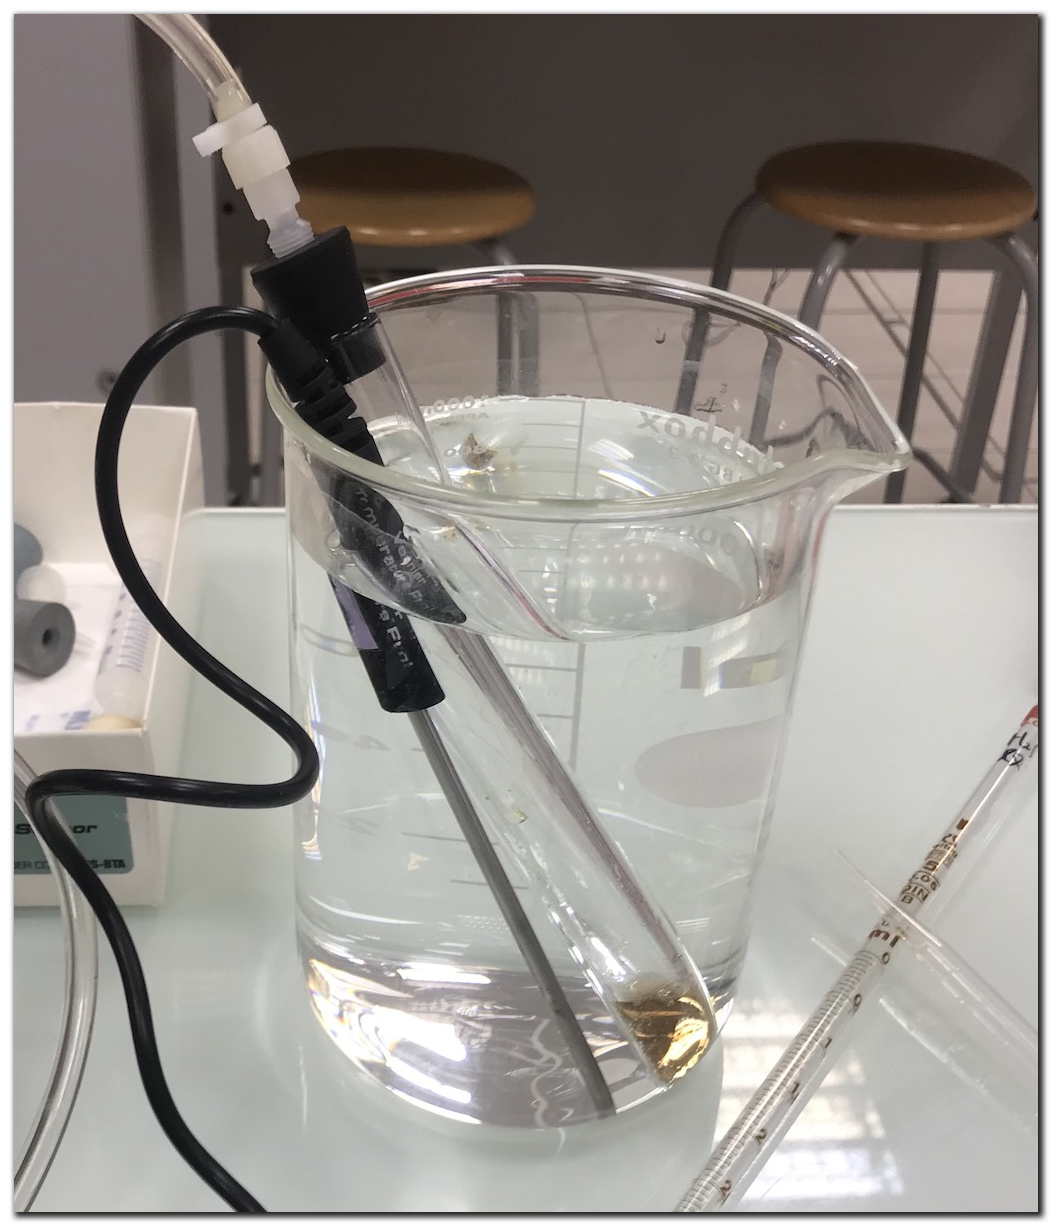
\includegraphics[width=0.5\textwidth]{imgs/setup}
    \caption{Setup of the experiment}
    \label{fig:setup}
\end{figure}


\section{Raw Data}
\begin{figure}[hbt]
  \centering
  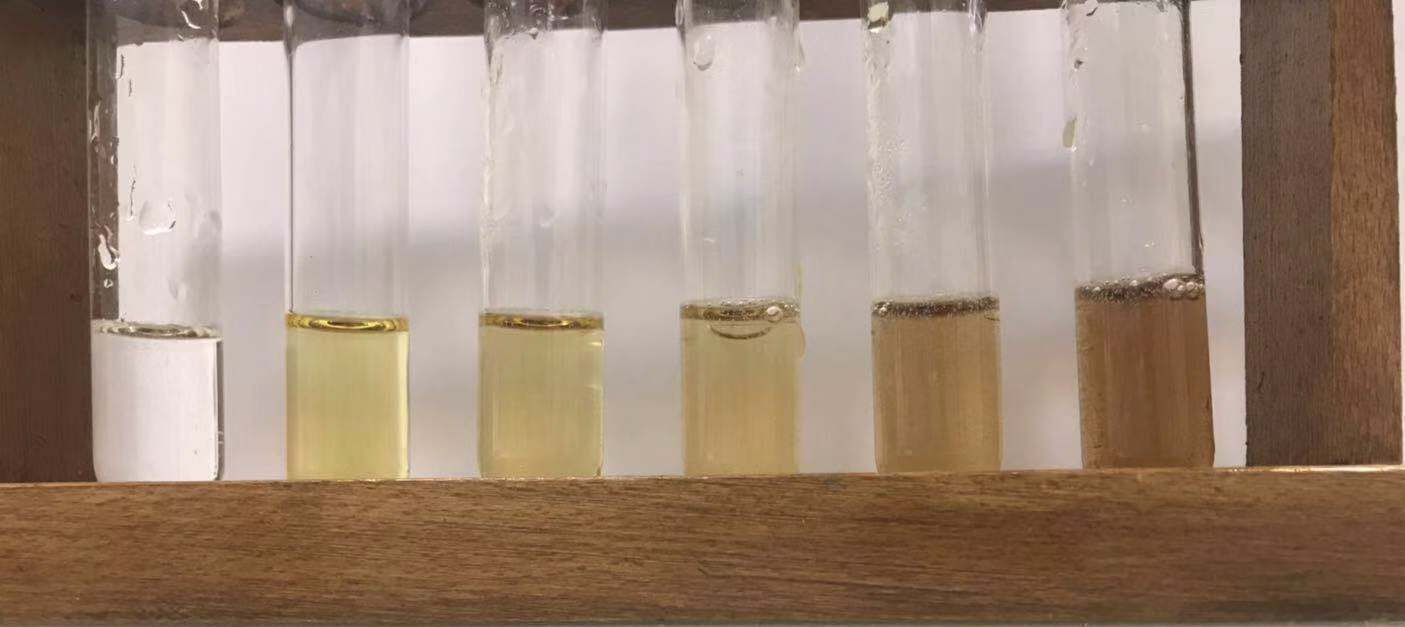
\includegraphics[width=\textwidth]{imgs/colours}
  \caption{Colours}
  \label{fig:colours}
\end{figure}


\section{Processed Data}

\section{Conclusion}

\section{Evaluation}

\section{Extension}

\printbibliography

\end{document}
